\section{Evaluation}

Here, we verify the effectiveness of our method through a usage scenario
demonstration and a formal user study.

\subsection{Usage Scenario: Analysis on MultiHop-RAG Dataset}

% \begin{figure*}
%     \centering
%     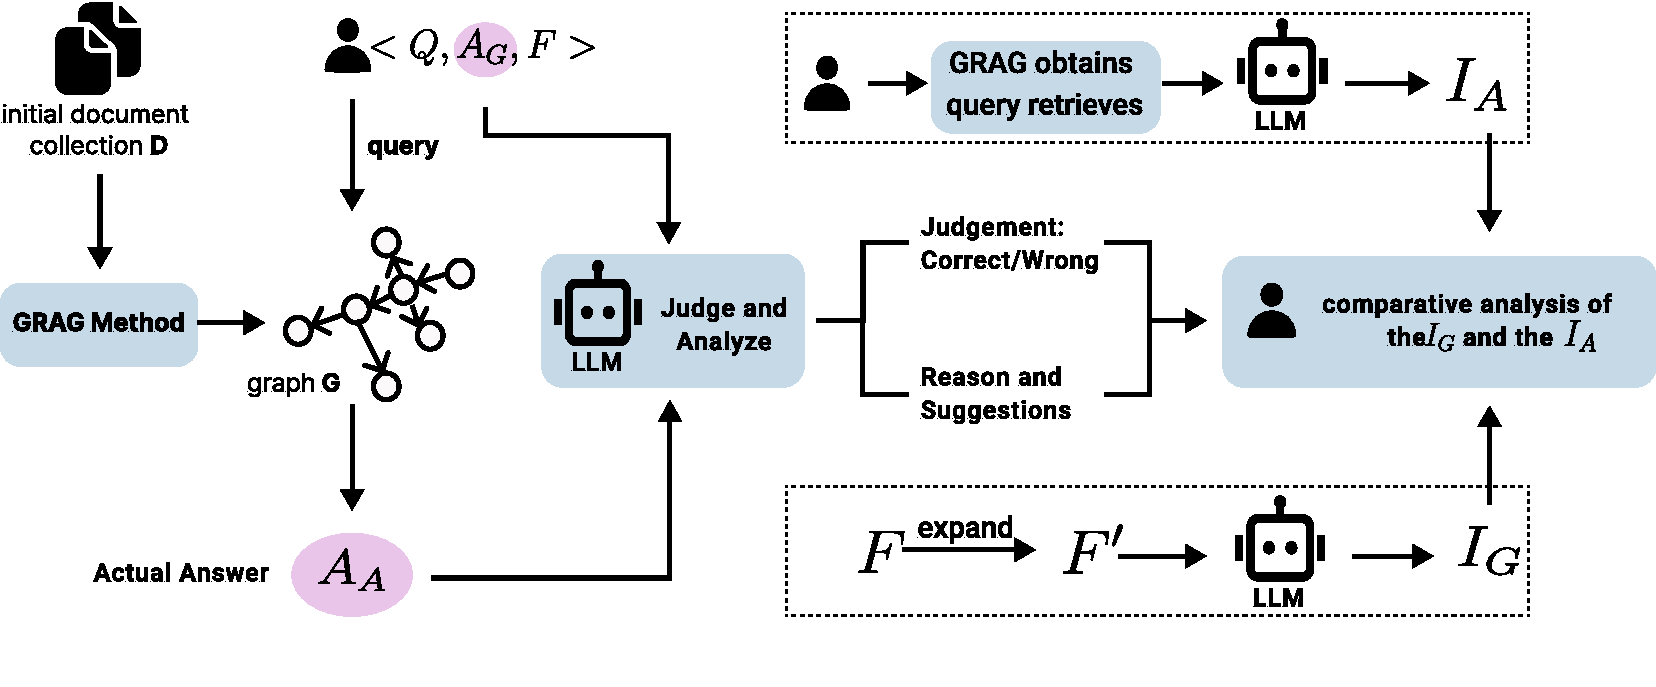
\includegraphics[width=\linewidth]{figs/Workflow.pdf}
%     \caption{Illustration of the system aiding in identifying and investigating graph issues.}
% \end{figure*}

This usage scenario illustrates how our system aids users in identifying and investigating issues related to graphs constructed by the GraphRAG system, thereby gaining insights into improving graph quality. Given the inherent complexity of the GraphRAG analysis process, we have also produced a demonstration video for this section to facilitate understanding.\footnote{Video URL: \url{https://gk0wk.github.io/XGraphRAG/}} The user employs the \textit{MultiHop-RAG} news dataset \cite{tang2024multihop} to construct a graph, intending to explore its quality and potential issues using our system.

The user inputs the query ``Which entity previously focused on illegal content and misinformation related to the Israel-Hamas conflict and is enforcing more than two pieces of legislation (act) in the digital domain?'' along with the Ground Truth Answer \textit{European Commission} and two key original text excerpts into the inference trace view for query and analysis.

Initially, the user observes that the entities \textit{Israel} and \textit{Hamas} were extracted from the query, ultimately leading to the answer \textit{Meta}. This answer is deemed \textit{wrong} by our system, which provides the reasoning for this judgment, highlighting two contradictions.

\begin{enumerate}
    \item \textit{Meta} is incorrectly identified as focusing on illegal content and misinformation about the \textit{Israel}-\textit{Hamas} conflict; this is actually the \textit{European Commission}'s role. (From Fact 1)
    \item \textit{Meta} is mistakenly thought to implement more than two digital acts, a responsibility that belongs to the \textit{European Commission}. (From Fact 2)
\end{enumerate}

It is noted that the query consists of two distinct parts: the first part tends to query the local association between explicit entities, while the second part aims to derive an answer based on a global summary topic. In this example, both parts result in contradictions, serving as an excellent illustration. Subsequently, the user investigates these two parts separately for local and global exploration.

\subsubsection{Exploration of Local Association Contradictions}

First, the reason why the segment ``Which entity previously focused on illegal content and misinformation related to the Israel-Hamas conflict'' failed to yield the correct answer should be analyzed. Issues with local queries can generally be attributed to a lack of entity or relationship information, so we will focus on exploring these two aspects.

By comparing inference steps, the user discovers that the steps related to \textit{Israel-Hamas} in the Actual Answer inference are steps 1, 3, 4, and 5. None of these steps utilized the \textit{European Commission} entity. However, in step 2 of the Ground Truth inference, entities such as \textit{Hamas} and \textit{European Commission} are used as recalls, indicating the presence of the \textit{European Commission} entity in the graph. Still, there is an omission when attempting to recall the \textit{European Commission} entity through \textit{Israel} and \textit{Hamas} entities.

Thus, the user seeks to explore whether there is a local association between the \textit{European Commission} and \textit{Israel} and \textit{Hamas}. In the Inference Trace View, the user right-clicks to recall the \textit{European Commission} entity and begins exploring its local relationships in the Entity Explore View. By hovering over \textit{Israel} and \textit{Hamas}, the user finds no highlighted edges or nodes in the Entity Explore View, indicating no direct relationship between \textit{Israel} and \textit{Hamas} with the \textit{European Commission}, resulting in a missing relationship on the graph.

Next, the user investigates the cause of the missing relationship. By left-clicking to recall the \textit{European Commission} entity in the Inference Trace View, the LLM Invocation View (for the merge stage) reveals the process of merging this entity from 11 raw entities. Hovering over ``Fact 1'' (a text segment describing the relationship between the \textit{European Commission} and \textit{Israel-Hamas}) in the Inference Trace View highlights one of the raw entities, indicating it originates from the chunk containing ``Fact 1''. However, the type and description of this raw entity are empty.

By clicking on ``Fact 1'', the LLM Invocation View (for the extraction stage) displays the chunks where the raw entity resides. It is found that the chunk does not extract any relationship with \textit{Israel} or \textit{Hamas}. Further reading of chunk text reveals that due to changes in subject and pronoun, the model fails to understand the relationship among the three, resulting in the failure of entity and relationship extraction and ultimately causing the loss of relational information.

\subsubsection{Exploration of Global Semantic Contradictions}

Next, the reason why the segment ``is enforcing more than two pieces of legislation (act) in the digital domain'' failed to yield the correct answer should be analyzed. Note that this answer originates from ``Fact 2'', where the \textit{European Commission} is responsible for enforcing the \textit{DMA} and \textit{DSA} digital acts on \textit{Meta}.

In the second step of the Actual Answer inference, information about \textit{Meta} fulfilling the \textit{DMA} and \textit{DSA} acts is indeed included, but the \textit{European Commission} is not mentioned. Further examination reveals that this inference step uses a topic report recall. Clicking on this topic recall, the LLM behavior analysis view shows the process of summarizing the topic into a report. Reading the report reveals descriptions of \textit{Meta}, the \textit{DSA}, and the \textit{DMA}, but no mention of the \textit{European Commission}. Further inspection of all entities and relationships used in this topic, hovering over ``Fact 2'', highlights entities and relationships related to ``Fact 2'' in the list, but the \textit{European Commission} is not found among them, indicating that the topic does not include the \textit{European Commission}, and there is no global semantic association between the \textit{European Commission} and the two acts.

Subsequently, the user further investigates the cause of semantic omission. In the previous analysis, the user suspected that the graph lacked the relationship from ``Fact 2'', which includes the \textit{European Commission} and the two acts. By left-clicking ``Fact 2'', the LLM Invocation View (for the extraction stage) displays the extraction process of the chunk. The user finds that although the chunk explicitly mentions the \textit{European Commission}'s responsibility for enforcing the two acts, the model fails to accurately capture this critical information during entity and relationship extraction. This discovery further confirms the user's previous suspicion that the LLM overlooked the extraction of the corresponding relationship.

\subsection{User Evaluation}
This study aims to evaluate the \textit{XGraphRAG} performance in analyzing \textit{GraphRAG} results, focusing on:

\begin{itemize}
\item \textbf{Efficiency}: The speed and simplification of analysis.
\item \textbf{Effectiveness}: The comprehensiveness and accuracy of the system's support.
\item \textbf{Usability}: The system's user-friendliness and ease of use.
\end{itemize}

It also compares \textit{XGraphRAG} with a baseline system for analysis support and user experience.
% This study aims to evaluate the performance of the \textit{XGraphRAG} system in assisting users with analyzing the results processed by \textit{GraphRAG}, focusing particularly on the following areas of enhancement.

% \begin{itemize}
%     \item \textbf{Efficiency}: The speed and simplification of analysis.
%     \item \textbf{Effectiveness}: The comprehensiveness and accuracy of the system's support.
%     \item \textbf{Usability}: The system's user-friendliness and ease of use.
% \end{itemize}

% Additionally, this study compares the overall improvements in analysis support and user experience between \textit{XGraphRAG} and a baseline system.

\subsubsection{Participants}
We invited 14 RAG engineers or experts as participants. These individuals have a thorough understanding of RAG principles but were not involved in the design requirements phase of this study, thereby enhancing the assessment's validity and the results' generalizability. Some have experience with naive RAG systems, while others are familiar with GraphRAG systems.

\subsubsection{Baseline Systems and Experimental Setup}

An additional baseline system was set up for comparative study \cite{feng2023promptmagician, feng2023xnli} alongside our system. Both systems are based on Microsoft's \textit{GraphRAG} \cite{edge2024local}, constructed using the \textit{MultiHop-RAG} dataset to build identical graphs, and utilize GPT-4 as the default LLM. The test dataset used in the experiments also comes from the \textit{MultiHop-RAG} dataset, including questions, answers, and graphs.

Baseline: We used \textit{Kotaemon}, a popular GraphRAG visualization interface system with high ratings on GitHub, as the baseline system. This system provides a visual question-and-answer interface for \textit{GraphRAG} \cite{edge2024local}, \textit{Nano-GraphRAG} \cite{gusye2024nanographrag}, \textit{LightRAG} \cite{guo2024lightrag}, and other systems. Users integrate GraphRAG for Q\&A through this system and display recalled entities, relationships, and topics referenced in the answers in the form of graph diagrams. It also shows various detailed information about recalls, such as explanations of entities. Users can click on entities and relationships in the graph to view the original chunk from which they originated.

Test Dataset: To test the ability of the GraphRAG system to handle both local and global questions, we improved the test questions of the test dataset. Firstly, we selected questions whose answers were names of people or organizations and ensured that these names had corresponding entities in the graph, with sufficient related text in the dataset. Then, we input these texts into the GPT-4 model to generate summary reports related to the entities. Subsequently, we verified the accuracy of the generated reports and posed global questions to them in a manner similar to the GraphRAG approach. Combining the original local questions, we formed the final test questions. Finally, to ensure the validity of the questions, we submitted these questions and related texts to three human experts for review. If the three experts could independently provide clear answers based on the texts and their answers were consistent, the question was deemed valid and could be used as a test case.

\subsubsection{Procedure and Tasks}

\textbf{Introduction (10 min):} We began by introducing the system to the participants, explaining the research motivation and methodology, and collecting basic information such as age and gender. With the participants' consent, we recorded and analyzed their usage behavior during subsequent tasks. Finally, we provided a detailed description of the features and characteristics of both the baseline system and the \textit{XGraphRAG} \cite{edge2024local} system, demonstrating their use through specific example scenarios.

\textbf{Task-based Analysis (60 min):} In this phase, participants interacted with both the baseline system and the \textit{XGraphRAG} \cite{edge2024local} system in a randomized order to eliminate any prior knowledge effects. The tasks were designed to assess the effectiveness and usability of each system, ensuring a fair level of complexity. We recorded the completion time and accuracy for each task to facilitate comparative analysis.

\textbf{Semi-structured Interview (30 min):} To further evaluate the interface design and usability of the systems, participants completed a questionnaire consisting of 6 items, using a five-point Likert scale to capture their perceptions and satisfaction. Participants rated each item from 1 (strongly disagree) to 5 (strongly agree). Concurrently, an open feedback session was conducted, allowing participants to explain the reasons behind their ratings and provide detailed insights into their user experience.

\subsubsection{Task Completion Analysis}

\begin{table}[h]
    \centering
    \makebox[\columnwidth][c]{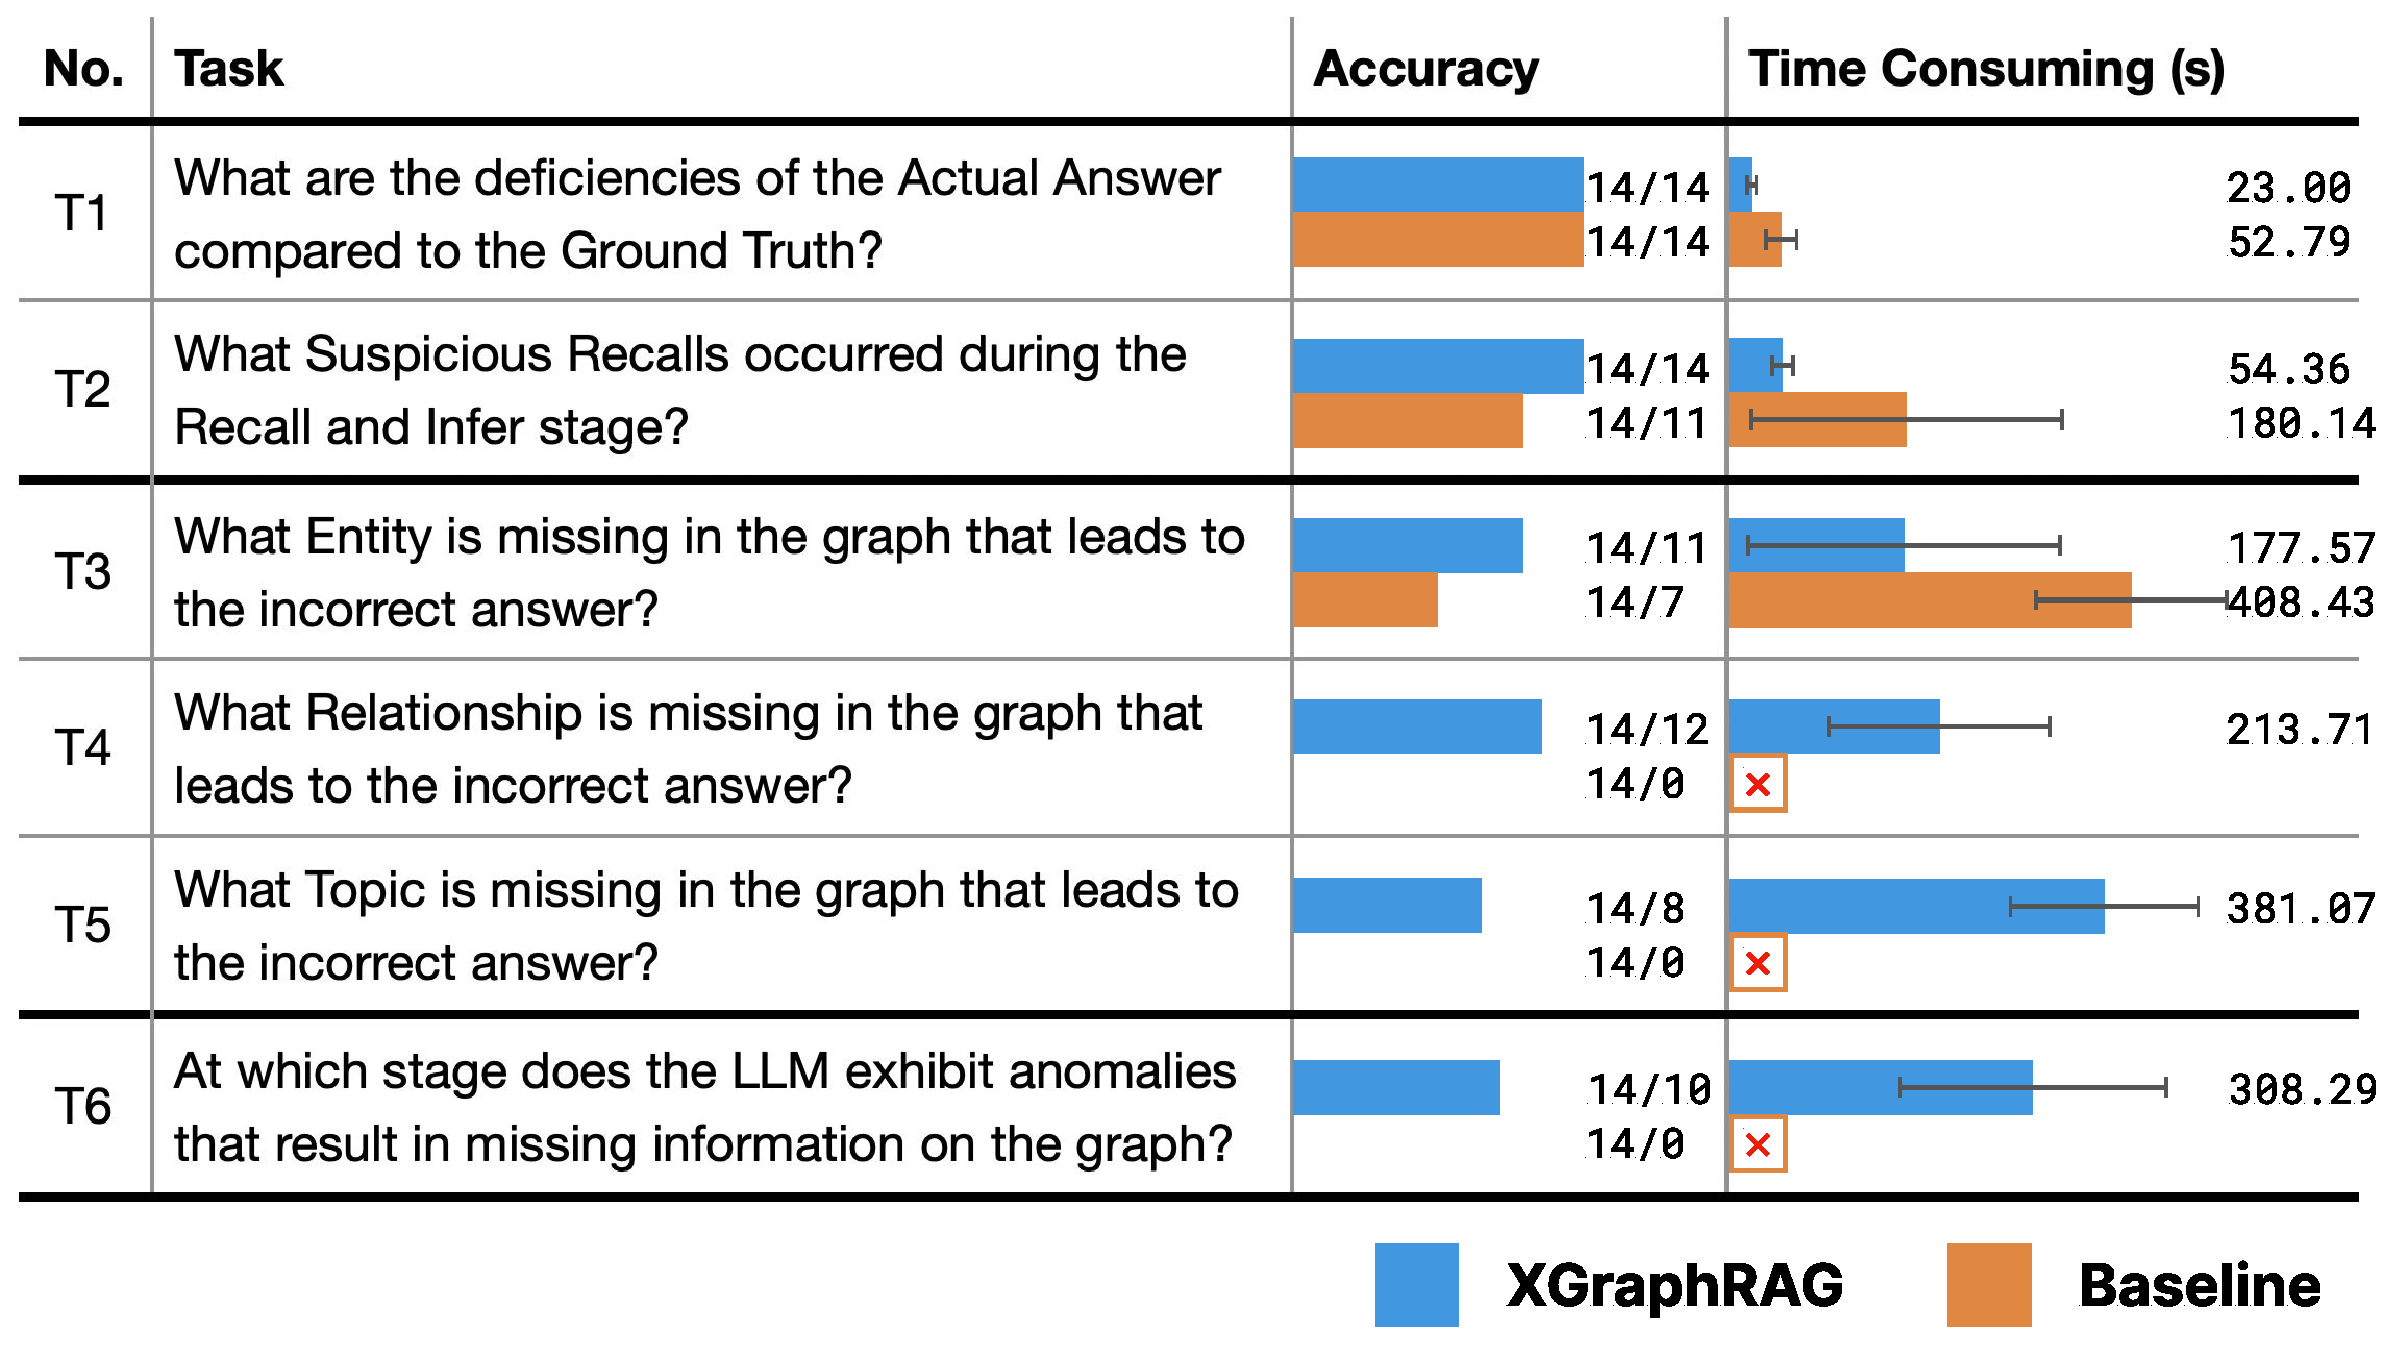
\includegraphics[width=1.05\columnwidth]{figs/Table1.pdf}}
    \caption{Accuracy and time consumption comparison result between XGraphRAG and the baseline system.}
    \label{tab:resultcompare}
\end{table}

For each task (T1-T6, in Table\ref{tab:resultcompare}) and each participant, we randomly assigned a test case to explore. Before starting any task, users are provided with all necessary prerequisite information and acknowledge that they understand it. For example, ``It is already known that the question was answered incorrectly because the Google entity was not recalled; please try to find information related to the missing Google entity.'' (Example of T3) and ``It is known that the relationship between Taylor Swift and Travis Kelce is missing in the chunk where Fact2 is located; please explore the reason.'' (Example of T6). Participants need to arrive at an answer within the stipulated time to consider the task complete, such as ``The relationship of Epic filing a monopoly lawsuit against Google in Fact1 is missing.'' (Answer to the example of T3).

Although participants varied in accuracy and time consumption in tasks, using \textit{XGraphRAG} significantly improved task accuracy while reducing time consumption. Below, we analyze each type of task and provide the setup of task problems and objectives.

\textbf{Analysis of Suspicious Recalls (T1 - T2)}: This set of tasks focuses on the system's ability to identify contradictions and suspicious recalls in the results and their locations. Compared to the baseline system, \textit{XGraphRAG} performed more efficiently and accurately. Its graphical interface allows participants to quickly highlight contradictions in retrieval results in T1, while enhanced visualization tools help locate suspicious recalls in T2, thus reducing the need for extensive manual review and improving diagnostic accuracy ($p_1=0.00012,\ p_2=0.00012$).

\textbf{Analysis of Missing Information (T3 - T5)}: This set of tasks emphasizes the system's ability to help participants identify missing information in the graph. Compared to the baseline system, \textit{XGraphRAG} significantly improved time efficiency and success rate, especially in T4 and T5, where the baseline system's inability to analyze relationships and topic reports posed a considerable challenge for participants in analyzing global relevance. The visual encoding in \textit{XGraphRAG} helps participants effectively locate areas of missing nodes or relationships. This design provides clear visual cues, significantly reducing the effort required to locate and analyze incomplete parts of the graph ($p_3=0.0033,\ p_4=0.0022,\ p_5=0.012$).

\textbf{Analysis of LLM Behavior (T6)}: In this task, the baseline system lacks the functionality to present and analyze the behavior of the GraphRAG framework model, unable to assist participants in tracking factors leading to missing information in the graph. Using \textit{XGraphRAG}, participants can effectively identify and analyze LLM behavior at various stages of the GraphRAG process and accurately pinpoint issues related to missing information ($p_6=0.0051$).

Overall, the \textit{XGraphRAG} system excels in both accuracy and time efficiency in task completion. These findings indicate that the enhanced visualization tools and graphical reasoning capabilities of \textit{XGraphRAG} significantly improve participant efficiency and accuracy in complex analytical scenarios.

\subsection{Semi-structured Interview Analysis}

\begin{table}[h]
    \centering
    \makebox[\columnwidth][c]{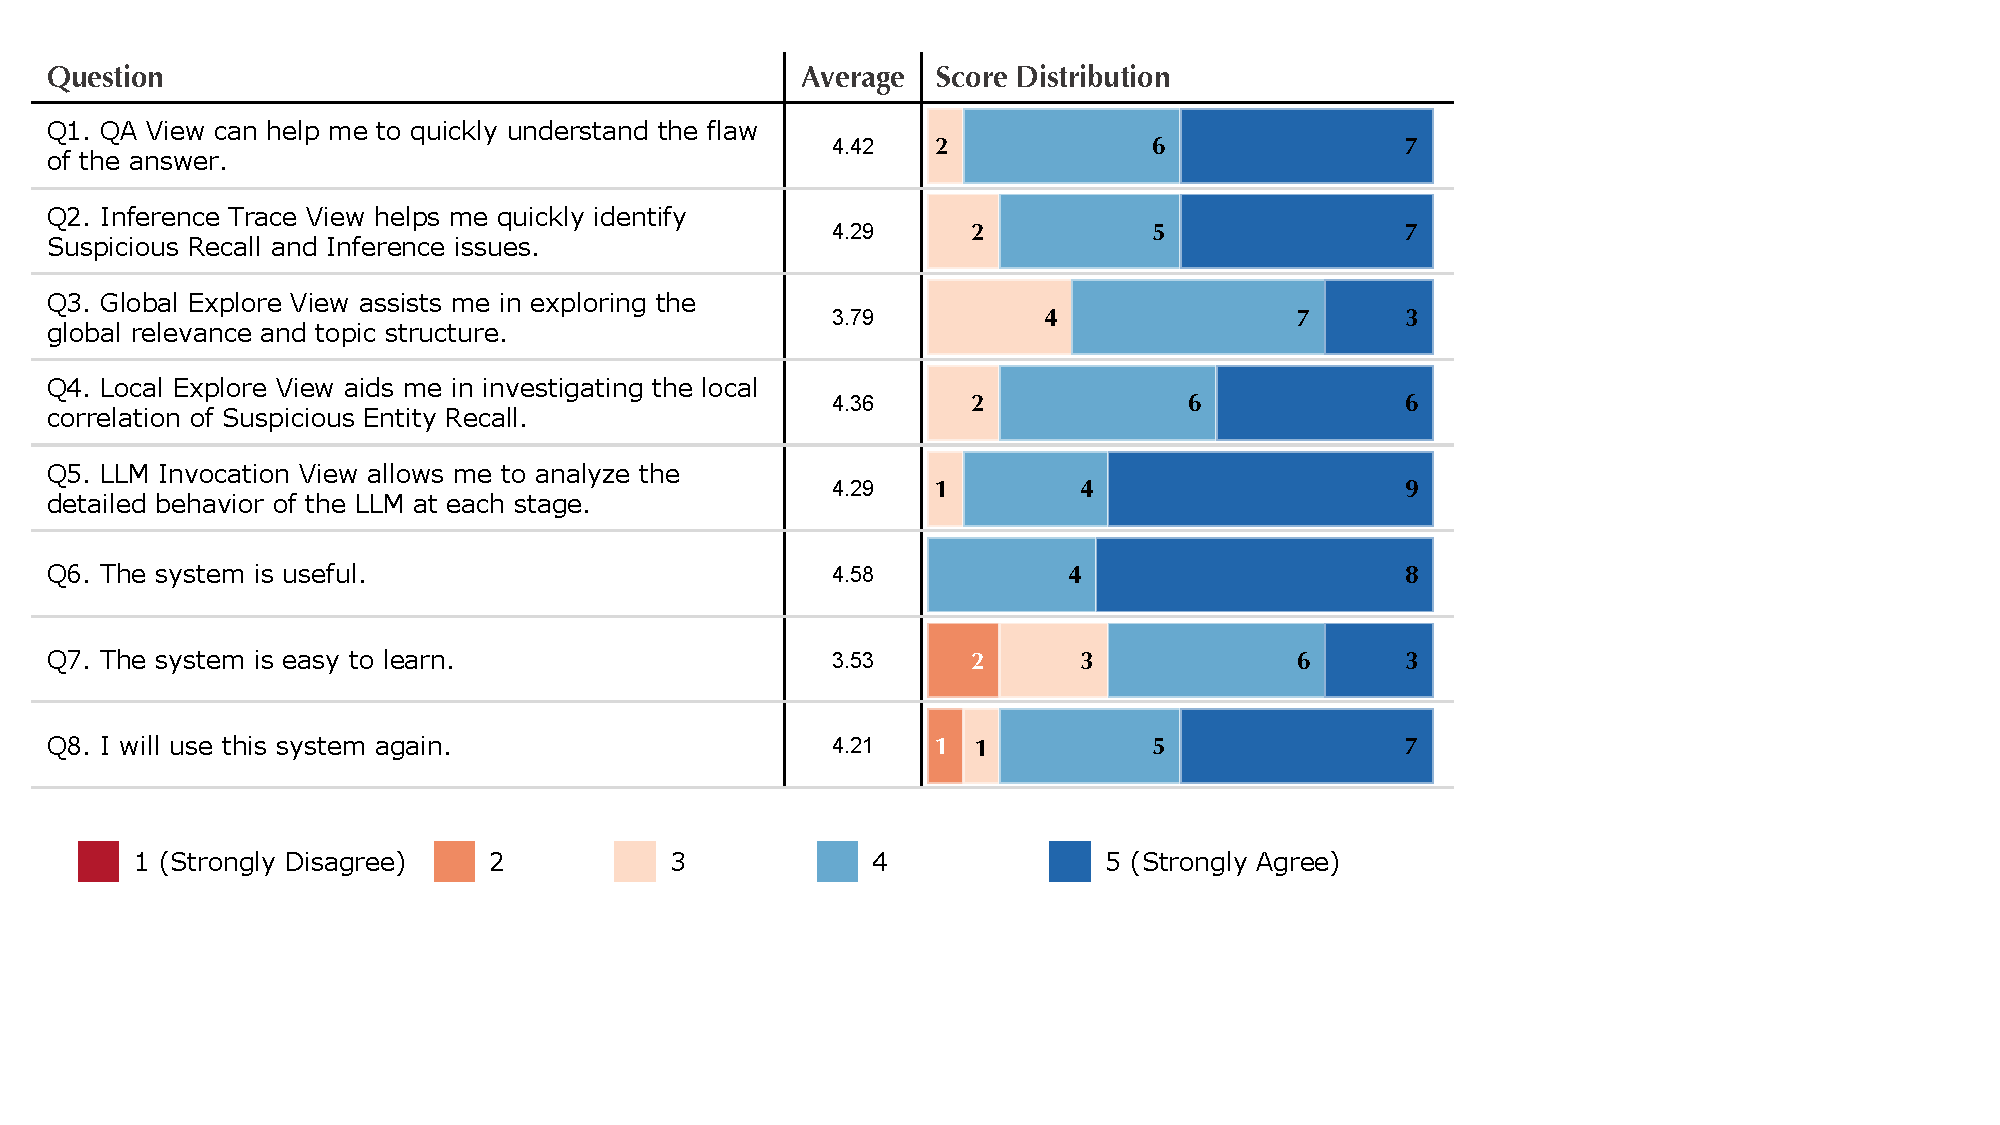
\includegraphics[trim={10pt 100pt 265pt 10pt}, clip,width=1\columnwidth]{figs/Table2.pdf}}
    \caption{The evaluation result for our system's effectiveness and usability.}
\vspace{-5pt}
\end{table}

We conducted a qualitative evaluation through semi-structured discussions to assess the system's usability and effectiveness. Participants were encouraged to provide detailed feedback on specific features, including their ability to identify reasoning process flaws, the clarity of visualizations, and the ease of interface interaction.

\textbf{Effectiveness:} All participants agreed that the Q\&A View effectively helped users quickly understand deficiencies in generated answers (Q1). P10 commented, ``The Q\&A View can automatically make judgments and provide reasons, along with three-point analysis suggestions, which greatly simplifies my thought process.'' P3 noted, ``In previous systems, I had to spend time reading the large outputs provided by the model, but now I can immediately see the key issues.''
Participants found the Inference Trace View particularly useful for identifying suspicious recalls and reasoning issues (Q2). P2 suggested providing an automatic translation feature for non-native speakers to accelerate understanding and analysis. P9 recommended integrating more context into the Inference Trace View, such as displaying additional information on mouse hover. P1 stated, ``Previously, I needed to use tools like neo4j to cross-system trace links for analysis, but now I can accomplish everything in one view, which gives me a sense of security.''
The Topic Explore View was highly praised for its assistance in exploring global correlations and corpus thematic structures (Q3). P8 emphasized, ``I've always wondered how to quickly understand what exactly a corpus is about, and this view has helped me; it's as important as a nautical chart.'' P11 stated, ``Even though the view is unnecessary for local problem analysis, I can quickly understand the distance between two unconnected entities by hovering over them, which is impressive and something I couldn't achieve with traditional graph tools.''
Participants also appreciated the Entity Explore View for its role in investigating local correlations of suspicious entity recalls (Q4). P13 pointed out, ``The view is simple and practical, allowing right-click expansion of entities for continuous exploration, and combined with the Topic Explore View, it enables targeted exploration.'' P1 suggested adding search filtering functionality to this view to handle large graphs.
The LLM Invocation View received positive feedback for its ability to analyze the detailed behavior of large language models at each stage (Q5). P5 stated, ``This is a missing link in GraphRAG and even RAG systems, and we need more interpretability work in LLM systems.'' P9 remarked, ``I want to understand the root cause of issues, and this view clearly shows each step, which is friendly to RAG developers; we no longer need to check lengthy run logs.''

\textbf{Usability:} Participants unanimously agreed that the system was useful for their tasks (Q6). P6 expressed, ``I previously tried tools like Kotaemon, but they only presented graph retrieval results, leaving a gap in presenting the complete chain from construction to retrieval reasoning, which made me reluctant to trust the model's answers. \textit{XGraphRAG} restored my confidence.''
Participants generally acknowledged the system's ease of use (Q7). We focused on feedback from participants who rated it 2 or 3. P2, P5, and others suggested adding a guided tutorial to help new users get started quickly. P7 mentioned, ``I hope there will be a mock example to guide users step-by-step through an analysis during their first use, which would enhance product usability.'' 
Most participants indicated they were likely to use the system again (Q8). Two low-scoring participants (Q8) acknowledged the system's functionality but had little need for diagnosing GraphRAG currently, so they were unsure about future use. P14 stated, ``XGraphRAG provides inspiration for designing subsequent Q\&A products in the industry and accelerates our development and testing processes.''